\documentclass[conference]{IEEEtran}
\IEEEoverridecommandlockouts

\usepackage{cite}
\usepackage{amsmath,amssymb,amsfonts}
\usepackage{algorithmic}
\usepackage{graphicx}
\usepackage{textcomp}
\usepackage{xcolor}
\usepackage{tabularx}
\usepackage{multirow}
\usepackage{array}
\usepackage{url}
\usepackage{microtype}

\def\BibTeX{{\rm B\kern-.05em{\sc i\kern-.025em b}\kern-.08em
    T\kern-.1667em\lower.7ex\hbox{E}\kern-.125emX}}

\begin{document}

\title{AI-Based Secure Online Voting System Using MERN Stack and Machine Learning}

\author{
\IEEEauthorblockN{K. Durga Charan}
\IEEEauthorblockA{\textit{Dept. of Computer Science \& Technology} \\
\textit{Madanapalle Inst. of Tech. \& Science}\\
Madanapalle, Andhra Pradesh, India \\
durgacharankondabathula@gmail.com}
\and
\IEEEauthorblockN{Pagadala Thanuja}
\IEEEauthorblockA{\textit{Dept. of Computer Science \& Technology} \\
\textit{Madanapalle Inst. of Tech. \& Science}\\
Madanapalle, Andhra Pradesh, India \\
pagadalathanujaa@gmail.com}
\and
\IEEEauthorblockN{Dhandu Shivani}
\IEEEauthorblockA{\textit{Dept. of Computer Science \& Technology} \\
\textit{Madanapalle Inst. of Tech. \& Science}\\
Madanapalle, Andhra Pradesh, India \\
shivanidhandu999@gmail.com}
\vspace{0.3cm}
\and
\IEEEauthorblockN{Pandrati Umesh}
\IEEEauthorblockA{\textit{Dept. of Computer Science \& Technology} \\
\textit{Madanapalle Inst. of Tech. \& Science}\\
Madanapalle, Andhra Pradesh, India \\
umesh63055@gmail.com}
\and
\IEEEauthorblockN{Paturu Vardhan Reddy}
\IEEEauthorblockA{\textit{Dept. of Computer Science \& Technology} \\
\textit{Madanapalle Inst. of Tech. \& Science}\\
Madanapalle, Andhra Pradesh, India \\
vardhan4036@gmail.com}
}

\maketitle

\begin{abstract}
Remote electronic voting systems face a critical trilemma: ensuring voter privacy (the secret ballot), enforcing strict eligibility without voter impersonation, and providing end-to-end auditability without introducing centralized points of compromise. In this paper, we design, implement, and evaluate an AI-augmented secure online voting architecture combining the MERN (MongoDB, Express.js, React, Node.js) web framework with a dedicated Python FastAPI machine learning microservice. Our system introduces a dual-tier security mechanism: (i) a multi-frame facial biometric authentication engine utilizing 128-dimensional illumination-invariant Discrete Cosine Transform (DCT) and spatial Sobel gradient descriptors paired with an eyeglass-resilient upper-face and Eye Aspect Ratio (EAR) liveness detector to prevent static spoofing; and (ii) an unsupervised Isolation Forest classifier analyzing five-dimensional session telemetry features to flag automated bot attacks, credential stuffing, and proxy anomalies in real time without disenfranchising voters. Cast ballots are recorded onto a linked SHA-256 cryptographic hash-chain ledger that guarantees append-only immutability and instant detection of database-level tampering, while identity-to-ballot decoupling preserves voter anonymity. Empirical evaluation on a held-out test distribution of 2,650 sessions demonstrates that the Isolation Forest achieves an overall accuracy of 97.06\%, an ROC-AUC of 0.9885, and an anomaly recall of 73.33\% with a low false positive rate of 1.52\%.
\end{abstract}

\begin{IEEEkeywords}
Electronic Voting, Biometric Authentication, Isolation Forest, Anomaly Detection, Cryptographic Hash-Chain Ledger, Anti-Spoofing, Liveness Detection, MERN Stack.
\end{IEEEkeywords}

\section{Introduction}
Remote electronic voting (e-voting) has long been proposed to increase democratic participation, reduce administrative overhead, and deliver rapid election certification \cite{mercuri2002better}. However, transitioning from physical polling stations to distributed web environments exposes the electoral process to severe attack vectors, including credential theft, automated ballot stuffing, session hijacking, presentation attacks using synthetic or printed media, and insider database manipulation \cite{springall2014security}.

Conventional web-based voting portals traditionally rely on single-factor or two-factor authentication (e.g., username/password paired with SMS or email One-Time Passwords). While One-Time Passwords (OTPs) mitigate basic credential reuse, they fail to defend against identity lending, credential selling, or coercion, as the physical identity of the individual operating the voting terminal remains unverified at the exact moment of ballot submission \cite{grassi2017nist}. Conversely, while biometric systems provide physical identity binding, naive implementations introduce significant usability hurdles (e.g., sensitivity to ambient lighting and failure on voters wearing spectacles) and vulnerability to presentation attacks (e.g., holding high-resolution photographs or digital displays to the camera) \cite{marcel2014handbook}. Furthermore, modern electoral threats increasingly employ automated bot scripts and proxy-hopping networks that mimic legitimate interactions at superhuman speeds, bypassing static access rules \cite{antonakakis2017understanding}.

To address these vulnerabilities simultaneously without sacrificing voter privacy or usability, we propose an integrated end-to-end architecture that combines web engineering with applied machine learning and cryptographic ledger verification. The core thesis of this work is that physical biometric verification and behavioral telemetry analysis must operate symbiotically: biometrics bind the voter's physical presence, while behavioral anomaly detection identifies automated orchestrations and illicit session anomalies.

The key contributions of this paper are:
\begin{itemize}
    \item \textbf{Dual-Tier AI Security Architecture:} We design and deploy a microservice-based architecture that decouples frontend user interactions (React 18) from core business logic (Express.js) and machine learning inference (FastAPI, scikit-learn, OpenCV), ensuring that resource-heavy biometric and telemetry calculations do not degrade portal availability.
    \item \textbf{Lighting-Invariant Biometrics with Eyeglass-Resilient Liveness:} We implement a 128-dimensional facial embedding engine combining 2D Discrete Cosine Transform (DCT) frequency coefficients and spatial Sobel gradient pooling. By zeroing the DC frequency component, the descriptor eliminates ambient lighting bias. We complement this with an anatomical upper-face band variance analysis that ensures robust liveness verification for voters wearing eyeglasses.
    \item \textbf{Unsupervised Behavioral Anomaly Detection:} We develop an Isolation Forest classifier trained on voter session telemetry (login frequency, IP volatility, voting duration, authentication failure ratios, and submission hour). Operating under a non-blocking administrative triage model, the classifier flags malicious bots (achieving an ROC-AUC of 0.9885) while ensuring that legitimate voters are not disenfranchised by false positives.
    \item \textbf{Cryptographic Hash-Chained Ledger with Identity Decoupling:} We enforce the secret ballot principle through a mathematical decoupling of voter eligibility records (\texttt{VoteRecord}) from anonymized ballots (\texttt{Ballot}). Every ballot is sealed onto a sequence-linked SHA-256 hash-chain ledger that allows independent Command Line Interface (CLI) verification of ledger continuity and immediate detection of database tampering.
    \item \textbf{Empirical Validation:} We report comprehensive experimental benchmarks on biometric inter/intra-class distance distributions, anti-spoofing performance, and session anomaly detection using reproducible metrics and confusion matrices.
\end{itemize}

\section{Related Work}

\subsection{Remote E-Voting Protocols and Security Properties}
Academic literature identifies several fundamental security properties required for any legally binding electoral system: \textit{eligibility} (only authorized voters can cast a vote), \textit{unreusability} (one-person-one-vote), \textit{ballot secrecy} (no entity can link a voter to their candidate choice), \textit{receipt-freeness} (voters cannot prove their choice to a third party for vote-buying or coercion), and \textit{individual and universal verifiability} (voters can verify their ballot was counted, and observers can verify the total tally) \cite{cortier2016election, benaloh1987verifiable}. 

Early systems like Helios \cite{adida2008helios} pioneered verifiable internet voting using homomorphic encryption and mix-nets. However, homomorphic schemes incur heavy computational overhead in distributed web clients and rely entirely on voter-side cryptographic key stewardship. When keys or credentials are compromised, homomorphic systems cannot determine whether the legitimate citizen or an unauthorized adversary cast the encrypted ballot.

\subsection{Biometric Authentication and Anti-Spoofing}
Facial recognition provides a non-invasive biometric modality for remote identity verification \cite{jain2007handbook}. Traditional deep convolutional neural networks (e.g., FaceNet \cite{schroff2015facenet}) achieve high verification rates under controlled lighting but require significant server-side GPU resources and often overfit to specific demographics and illumination angles. To maintain low-latency inference on commodity hardware, spatial-frequency descriptors utilizing Discrete Cosine Transform (DCT) and gradient histograms have emerged as computationally efficient alternatives \cite{hafed2001face}.

To prevent presentation attacks (holding photographs or recorded videos to the webcam), Presentation Attack Detection (PAD) methods analyze micro-textures, temporal motion, or physiological signals such as eye blinks \cite{patel2015live}. Soukupov{\'a} and {\v{C}}ech \cite{soukupova2016real} formalized the Eye Aspect Ratio (EAR) metric based on facial landmarks to monitor blink patterns. However, standard facial landmark and Haar cascade detectors suffer high failure rates when users wear spectacles due to glare and lens rim occlusion \cite{viola2004robust}. Our work addresses this limitation by supplementing EAR with an anatomical upper-face band variance metric.

\subsection{Behavioral Anomaly Detection for Fraud Prevention}
Electoral platforms face automated botnets, credential stuffing, and coordinated Sybil attacks \cite{douceur2002sybil}. Traditional intrusion detection systems (IDS) rely on signature-based matching, which fails against novel attack patterns or slow-rate distributed botnets \cite{debar1999towards}. Machine learning approaches model normal user behavior and detect deviations. 

Liu et al. \cite{liu2008isolation, liu2012isolation} introduced the Isolation Forest algorithm, demonstrating that anomalies can be isolated using fewer random recursive axis-aligned splits than nominal data points. Unlike distance-based or density-based clustering algorithms that scale quadratically with dataset size, Isolation Forest exhibits linear time complexity and low memory requirements, making it ideal for real-time web telemetry inspection.

\subsection{Blockchain and Hash-Chained Ledgers in E-Voting}
Distributed Ledger Technology (DLT) and blockchain architectures have been widely investigated for auditable voting \cite{kshetri2018blockchain, crosby2016blockchain}. While public proof-of-work (PoW) or proof-of-stake (PoS) blockchains guarantee decentralization, they introduce scalability bottlenecks, transaction fees, high latency, and the risk that public transaction ledgers leak voter participation timestamps \cite{park2021going}. 

Consequently, several researchers propose permissioned, lightweight append-only cryptographic ledgers using backward hash chaining (similar to certificate transparency logs) \cite{laurie2014certificate}. Each ballot block references the cryptographic hash of its predecessor, creating a tamper-evident sequence that detects retroactive record insertion, modification, or deletion while avoiding the computational overhead of decentralized consensus networks.

\section{System Architecture}
The proposed platform adopts a decoupled multi-tier microservice architecture designed to isolate heavy computational workloads (computer vision and machine learning inference) from transaction processing and user interface rendering.

\subsection{Microservice Separation \& Inter-Service Security}
The system is partitioned into two distinct backend services:
\begin{enumerate}
    \item \textbf{Core Application Server (Node.js/Express.js):} Manages user registration, session management, relational integrity between voter eligibility and cryptographic ledgers, and electoral governance rules.
    \item \textbf{Machine Learning Microservice (Python 3.11/FastAPI):} Exposes stateless endpoints for biometric feature extraction (\texttt{/api/ml/extract-embedding}), face verification (\texttt{/api/ml/verify-face}), liveness verification (\texttt{/api/ml/liveness-check}), and session fraud detection (\texttt{/api/ml/detect-fraud}).
\end{enumerate}

To secure service-to-service communication across the internal network, all calls from the Node.js core to the FastAPI service require a shared internal service secret (\texttt{INTERNAL\_SERVICE\_KEY}) passed in the HTTP request header. Direct public requests to the ML microservice are dropped by firewall rules, mitigating external denial-of-service and model manipulation attacks.

\subsection{Operational Lifecycle Pipeline}
The operational lifecycle encompasses four sequential stages:
\begin{enumerate}
    \item \textbf{Voter Registration and KYC:} The user submits legal identity attributes, establishes a password, and captures an enrollment facial photograph via the live webcam. The backend delegates the image to the ML service, which extracts a canonical 128-dimensional biometric embedding. An email OTP is dispatched via SMTP. Upon OTP verification, the voter account enters a \texttt{pending} state awaiting administrative KYC authorization.
    \item \textbf{Administrative Identity Verification:} An election official reviews the citizen's government voter ID and webcam photograph in the administrative dashboard, updating the voter's status to \texttt{approved} or \texttt{rejected}.
    \item \textbf{Ballot Access and Biometric Challenge:} When an approved voter initiates ballot submission, the client interface activates a multi-frame burst capture (4 frames over 1.2 seconds). The ML service verifies both physical liveness (anti-spoofing) and biometric matching against the registered embedding ($d \le 0.76$). Concurrently, client-side session telemetry is harvested.
    \item \textbf{Cryptographic Ledger Sealing:} If biometric verification succeeds, the core server executes an atomic database operation: (i) it verifies and writes a \texttt{VoteRecord} enforcing the one-person-one-vote constraint; (ii) it queries the latest block of the election's ledger; (iii) it computes the SHA-256 hash chaining to the previous block; (iv) it persists the anonymized \texttt{Ballot}; and (v) it runs the telemetry vector through the Isolation Forest, logging a \texttt{FraudAlert} if anomalous behavior is identified.
\end{enumerate}

\section{Methodology \& Technical Formulation}

\subsection{Tier-1 Access Control: Multi-Factor Authentication}
Authentication relies on a defense-in-depth scheme:
\begin{itemize}
    \item \textbf{Password Hashing:} Passwords are salted and hashed using bcrypt with an adaptive work factor of 12 iterations:
    \begin{equation}
        \text{Hash} = \text{bcrypt}(\text{Password}, \text{Salt}_{12})
    \end{equation}
    \item \textbf{Email Verification via Salted OTP:} Registration triggers the generation of a cryptographically secure 6-digit pseudo-random integer $R \in [100000, 999999]$. Rather than persisting the plaintext OTP, the database stores an expiration timestamp $T_{\text{exp}} = T_{\text{current}} + 10\text{ min}$ and an HMAC-SHA-256 hash digest:
    \begin{equation}
        H_{\text{OTP}} = \text{HMAC-SHA256}(R, K_{\text{jwt\_secret}})
    \end{equation}
    \item \textbf{Dual-Token Session Architecture:} Upon authentication, the client receives a short-lived Access Token (15 minutes) and a long-lived Refresh Token (7 days) submitted to obtain new session tokens without re-entering credentials.
\end{itemize}

\subsection{Biometric Feature Representation: 128-d DCT/Sobel Spatial-Frequency Descriptors}
To extract a facial biometric representation that is invariant to illumination while maintaining fast CPU-only inference, we formulate a 128-dimensional hybrid frequency-spatial descriptor:
\begin{enumerate}
    \item \textbf{Face Normalization:} The input frame is converted to grayscale, equalized via Contrast Limited Adaptive Histogram Equalization (CLAHE, clip limit = 2.0, grid = $8 \times 8$), and processed by a Haar cascade detector to isolate the primary face bounding box. The cropped face region is normalized to a fixed resolution of $128 \times 128$ pixels.
    \item \textbf{Frequency Domain Transformation (DCT):} A 2D Discrete Cosine Transform (DCT-II) is applied to the normalized floating-point grayscale image $I(x, y)$:
    \begin{equation}
    \begin{split}
        D(u, v) = \alpha(u)\alpha(v) \sum_{x=0}^{N-1}\sum_{y=0}^{N-1} I(x, y) & \cos\left[\frac{\pi(2x+1)u}{2N}\right] \\
        & \times \cos\left[\frac{\pi(2y+1)v}{2N}\right]
    \end{split}
    \end{equation}
    where $N=128$, and the orthonormal scaling factor $\alpha(\cdot)$ is:
    \begin{equation}
        \alpha(u) = \begin{cases} 
        \sqrt{\frac{1}{N}}, & u = 0 \\ 
        \sqrt{\frac{2}{N}}, & u \ge 1 
        \end{cases}
    \end{equation}
    \item \textbf{Lighting Invariance via DC Zeroing:} The top-left $8 \times 8$ low-to-mid frequency coefficients capturing fundamental structural facial topology are extracted. Crucially, the direct current coefficient $D(0, 0)$—which represents average global surface luminance—is set to zero:
    \begin{equation}
        \mathbf{f}_{\text{DCT}} = \left[0.0, \, D(0, 1), \, D(0, 2), \, \dots, \, D(7, 7)\right]^T \in \mathbb{R}^{64}
    \end{equation}
    The vector is unit-normalized: $\hat{\mathbf{f}}_{\text{DCT}} = \mathbf{f}_{\text{DCT}} / \|\mathbf{f}_{\text{DCT}}\|_2$.
    \item \textbf{Spatial Gradient Pooling:} In parallel, horizontal ($G_x$) and vertical ($G_y$) Sobel gradient operators are convolved with the equalized image to compute the edge magnitude map:
    \begin{equation}
        M(x, y) = \sqrt{G_x(x, y)^2 + G_y(x, y)^2}
    \end{equation}
    The magnitude map is partitioned into an $8 \times 8$ regular grid (cell size $16 \times 16$ pixels). The mean gradient intensity of each cell $k$ ($1 \le k \le 64$) is computed and normalized:
    \begin{equation}
        \hat{\mathbf{f}}_{\text{Sobel}} = \frac{\mathbf{f}_{\text{Sobel}}}{\|\mathbf{f}_{\text{Sobel}}\|_2} \in \mathbb{R}^{64}
    \end{equation}
    \item \textbf{Canonical 128-d Vector Concatenation:} The composite embedding $\mathbf{v} \in \mathbb{R}^{128}$ is formed by concatenating both 64-dimensional feature representations and applying global $L_2$-normalization:
    \begin{equation}
        \mathbf{v} = \frac{\left[\hat{\mathbf{f}}_{\text{DCT}}^T, \; \hat{\mathbf{f}}_{\text{Sobel}}^T\right]^T}{\left\|\left[\hat{\mathbf{f}}_{\text{DCT}}^T, \; \hat{\mathbf{f}}_{\text{Sobel}}^T\right]^T\right\|_2} \in \mathbb{R}^{128}
    \end{equation}
    \item \textbf{Biometric Distance Formulation:} Verification compares a live query embedding $\mathbf{u}$ against the registered KYC template $\mathbf{v}$ using Euclidean distance:
    \begin{equation}
        d(\mathbf{u}, \mathbf{v}) = \|\mathbf{u} - \mathbf{v}\|_2 = \sqrt{\sum_{i=1}^{128}(u_i - v_i)^2}
    \end{equation}
    A candidate identity is verified if and only if $d(\mathbf{u}, \mathbf{v}) \le \tau_{\text{match}}$, where the operational decision threshold is calibrated to $\tau_{\text{match}} = 0.76$.
\end{enumerate}

\subsection{Presentation Attack Detection (Liveness Analysis)}
To defeat presentation attacks using static physical paper cutouts, smartphone displays, or photographs, the system captures a temporal burst of $K=4$ frames at 300 ms intervals ($t \in [0.0, 1.2\text{ s}]$). The verification pipeline evaluates two physiological properties:
\begin{enumerate}
    \item \textbf{Temporal Optical Micro-Motion:} For consecutive normalized face crops $C_0$ and $C_{K-1}$, the mean absolute pixel difference across all color channels is evaluated:
    \begin{equation}
        \Delta_{\text{motion}} = \frac{1}{W \cdot H \cdot C} \sum_{x=1}^{W}\sum_{y=1}^{H}\sum_{c=1}^{C} |C_0(x, y, c) - C_{K-1}(x, y, c)|
    \end{equation}
    While static photographs yield $\Delta_{\text{motion}} < 0.35$ due to absence of biological motion, genuine human presence generates micro-movements, breathing variance, and optical sensor fluctuations ($\Delta_{\text{motion}} \ge 0.60$).
    \item \textbf{Anatomical Upper-Face Band Variance (Eyeglass-Resilient Liveness):} Standard Eye Aspect Ratio (EAR) algorithms fail when voters wear spectacles due to reflections and frame occlusion. Our system defines an anatomical upper-face sub-region $\Omega$ spanning the vertical interval $y \in [0.20 H_f, 0.52 H_f]$ and horizontal interval $x \in [0.15 W_f, 0.85 W_f]$ of the detected face bounding box. When cascade eye detection succeeds, the Eye Aspect Ratio (EAR) is computed from the vertical-to-horizontal gradient ratio:
    \begin{equation}
        \text{EAR} \approx 0.25 \times \frac{\mu\left(|G_y|\right)}{\mu\left(|G_x|\right) + \epsilon}
    \end{equation}
    where $\epsilon = 10^{-6}$. When cascade eye detection fails due to spectacles, the system evaluates the temporal texture difference across the anatomical eye band: $\Delta_{\text{band}} = \mu(|B_0 - B_{K-1}|)$. Liveness is confirmed if any of the following conditions hold: (i) at least one distinct blink event is observed; (ii) $\Delta_{\text{band}} \ge 0.55$; (iii) $\Delta_{\text{motion}} \ge 0.60$; or (iv) EAR temporal variance $\sigma^2_{\text{EAR}} \ge 0.00003$.
\end{enumerate}

\subsection{Behavioral Anomaly Detection: Unsupervised Isolation Forest}
Automated voting scripts, credential-stuffing tools, and coordinated botnets exhibit distinct statistical signatures in their session interaction telemetry. We model this behavior using an unsupervised Isolation Forest ensemble \cite{liu2008isolation}.

Each voting transaction collects a 5-dimensional telemetry vector $\mathbf{x} = [x_1, x_2, x_3, x_4, x_5]^T$:
\begin{itemize}
    \item $x_1$: \texttt{login\_frequency\_24h} (Integer) --- Total logins recorded in past 24 hours.
    \item $x_2$: \texttt{ip\_change\_count} (Integer) --- Number of unique IP addresses associated with session token.
    \item $x_3$: \texttt{time\_to\_vote\_seconds} (Float) --- Time elapsed between ballot booth rendering and final submission.
    \item $x_4$: \texttt{failed\_attempts\_ratio} (Float $\in [0, 1]$) --- Ratio of prior invalid authentication attempts to total attempts.
    \item $x_5$: \texttt{hour\_of\_day} (Float $\in [0, 24]$) --- Local diurnal time of ballot casting.
\end{itemize}

The feature vector is normalized using standard score scaling: $z_j = (x_j - \mu_j) / \sigma_j$. The anomaly score $s(\mathbf{z}, \psi)$ across an ensemble of $n_{\text{tree}} = 100$ isolation trees is formulated as:
\begin{equation}
    s(\mathbf{z}, \psi) = 2^{-\frac{\mathbb{E}(h(\mathbf{z}))}{c(\psi)}}
\end{equation}
where $h(\mathbf{z})$ denotes the path length (number of edges traversed from root to terminating leaf node in a given tree), $\mathbb{E}(h(\mathbf{z}))$ is the expectation of $h(\mathbf{z})$ across all 100 trees, and $c(\psi)$ is the average path length of unsuccessful searches in a Binary Search Tree (BST) given subsample size $\psi$:
\begin{equation}
    c(\psi) = 2\left(\ln(\psi - 1) + \gamma\right) - \frac{2(\psi - 1)}{\psi}
\end{equation}
where $\gamma \approx 0.5772156649$ is the Euler-Mascheroni constant, and $\psi = 256$ is the subsampling size. Anomalies are flagged whenever the decision function evaluates to negative: $f(\mathbf{z}) = -s(\mathbf{z}, \psi) - \text{offset} < 0$.

\subsection{Cryptographic Hash-Chained Ledger \& Strict Decoupling}

\subsubsection{Identity-to-Ballot Decoupling (Secret Ballot Principle)}
To guarantee ballot privacy, the system strictly separates voter identity tracking from the recorded ballot across two collections:
\begin{itemize}
    \item \texttt{VoteRecord}: Contains \texttt{\{voterId, electionId, receiptHash, timestamp\}}. A compound unique index on \texttt{\{voterId: 1, electionId: 1\}} guarantees that any attempt by a voter to cast more than one ballot in the same election triggers a database-level duplicate key exception (HTTP 409), enforcing the one-person-one-vote rule.
    \item \texttt{Ballot}: Contains \texttt{\{electionId, candidateId, receiptHash, sequenceNumber, previousHash, blockHash, timestamp\}}. No user identifier, IP address, or session identifier is stored. The only shared attribute is \texttt{receiptHash}:
    \begin{equation}
        \text{Receipt} = \text{"REC-"} \,\|\, \text{SHA256}(\text{voterId} \,\|\, \text{electionId} \,\|\, \text{salt})[:12]
    \end{equation}
    The receipt confirms ballot inclusion on the public ledger without disclosing the candidate selected, fulfilling receipt-freeness.
\end{itemize}

\subsubsection{Linked SHA-256 Ledger Chaining}
Each election maintains an independent append-only cryptographic ledger initialized with a Genesis block:
\begin{equation}
    \text{Hash}_0 = \text{SHA256}\left(\text{"GENESIS\_BLOCK\_"} \,\|\, \text{electionId} \,\|\, t_0\right)
\end{equation}
For every subsequent ballot $k \ge 1$, the block hash is computed strictly over the canonical concatenation:
\begin{equation}
\begin{split}
    \text{Hash}_k = \text{SHA256}\Big(& \text{Hash}_{k-1} \,\|\, \text{electionId} \,\|\, \text{candidateId} \\
    & \|\, t_k \,\|\, \text{Receipt}_k \Big), \quad \forall k \ge 1
\end{split}
\end{equation}
where $\text{Hash}_{k-1}$ is the exact \texttt{blockHash} of sequence block $k-1$. If an insider with administrative database access modifies candidate $c_k$ or timestamp $t_k$ in Block $k$, then $\text{SHA256}(\text{Block}_k) \neq \text{Block}_{k+1}.\text{previousHash}$, permanently breaking backward continuity from block $k+1$ through the tip of the chain.

\section{Implementation Details}
\begin{itemize}
    \item \textbf{Client Frontend:} Built on React 18, Vite, and Tailwind CSS. Biometric capture utilizes \texttt{react-webcam} capturing high-definition frames rendered onto a real-time HTML5 canvas with dynamic oval guides.
    \item \textbf{Core Application Server:} Express.js on Node.js v20.18.0. Includes Mongoose ODM, Helmet HTTP headers, CORS whitelisting, and JSON Web Token verification.
    \item \textbf{ML Service:} FastAPI on Python 3.11.9, utilizing OpenCV 4.10, NumPy, scikit-learn 1.5, and \texttt{joblib}.
    \item \textbf{Database:} MongoDB 8.3 Enterprise server configured with write concerns and compound indices on electoral keys.
\end{itemize}

\subsection{Administrative Real-Time Fraud Triage}
When the Isolation Forest or biometric engine identifies an anomaly, the transaction is handled under a \textbf{non-blocking policy}:
\begin{itemize}
    \item The ballot is successfully chained to the ledger so that legitimate citizens are not disenfranchised by occasional algorithmic false alarms.
    \item Simultaneously, a \texttt{FraudAlert} document is persisted with status \texttt{FLAGGED}, storing the anomaly score, Euclidean biometric distance, and exact session telemetry features.
    \item The Administrative Dashboard displays live flagged alerts with visual badges, permitting election officials to review anomalous voting sessions, cross-reference IP rotation patterns, and conduct post-election forensic audits.
\end{itemize}

\subsection{Self-Service Account Erasure \& Administrative Removal}
To satisfy modern data privacy frameworks (e.g., GDPR Right to Erasure / Article 17) \cite{gdpr2016regulation}, the system implements authenticated voter account deletion via \texttt{DELETE /api/v1/auth/me} and administrative deletion via \texttt{DELETE /api/v1/admin/voters/:id}. Previously cast anonymized ballots remain permanently anchored on the immutable hash-chain ledger without orphaning blocks, preserving election tally integrity while honoring voter privacy.

\section{Experimental Setup and Results}

\subsection{Dataset Synthesis \& Telemetry Distributions}
Because live production telemetry containing confirmed malicious electoral attacks cannot be ethically harvested without prior deployment, an empirical dataset generator was engineered in \texttt{ml-service/training/generate\_synthetic\_data.py}. The generator models $N_{\text{normal}} = 8,000$ legitimate voter records and $N_{\text{anomaly}} = 400$ malicious/bot records (4.76\% contamination). Table \ref{tab:telemetry} details the parameter ranges across both distributions.

\begin{table}[htbp]
\caption{Telemetry Feature Definitions and Empirical Parameter Ranges}
\label{tab:telemetry}
\centering
\renewcommand{\arraystretch}{1.25}
\resizebox{\columnwidth}{!}{%
\begin{tabular}{|c|l|c|c|}
\hline
\textbf{Index} & \textbf{Telemetry Feature} & \textbf{Human Range} & \textbf{Malicious / Bot Range} \\
\hline
$x_1$ & \texttt{login\_freq\_24h} & $[1, 3]$ ($\lambda=1.2$) & $[10, 60]$ ($\lambda=25.0$) \\
\hline
$x_2$ & \texttt{ip\_change\_count} & $[0, 1]$ ($\lambda=0.1$) & $[3, 15]$ ($\lambda=6.0$) \\
\hline
$x_3$ & \texttt{time\_to\_vote\_seconds} & $[15.0, 180.0]$ ($\mu=45.0\text{ s}$) & $[0.5, 3.0]$ ($\mu=1.2\text{ s}$) \\
\hline
$x_4$ & \texttt{failed\_attempts\_ratio} & $[0.0, 0.1]$ ($\mu=0.02$) & $[0.4, 1.0]$ ($\mu=0.75$) \\
\hline
$x_5$ & \texttt{hour\_of\_day} & $[8.0, 22.0]$ (Diurnal) & $[1.0, 5.0]$ (Nocturnal Burst) \\
\hline
\end{tabular}%
}
\end{table}

\subsection{Anomaly Detection Performance}
The Isolation Forest model was evaluated on a strictly isolated test partition of 2,650 sessions (2,500 normal samples, 150 anomalous samples). Table \ref{tab:confusion} presents the resulting confusion matrix with complete grid lines.

\begin{table}[htbp]
\caption{Isolation Forest Confusion Matrix on Test Partition ($N = 2,650$)}
\label{tab:confusion}
\centering
\renewcommand{\arraystretch}{1.3}
\begin{tabular}{|l|c|c|c|}
\hline
\textbf{Ground Truth} & \textbf{Pred. Normal} & \textbf{Pred. Anomaly} & \textbf{Class Total} \\
\hline
\textbf{Actual Normal} & \textbf{2,462} ($TN$) & \textbf{38} ($FP$) & 2,500 \\
\hline
\textbf{Actual Anomaly} & \textbf{40} ($FN$) & \textbf{110} ($TP$) & 150 \\
\hline
\textbf{Total Predicted} & \textbf{2,502} & \textbf{148} & \textbf{2,650} \\
\hline
\end{tabular}
\end{table}

\begin{table}[htbp]
\caption{Anomaly Detection Empirical Performance Metrics}
\label{tab:metrics}
\centering
\renewcommand{\arraystretch}{1.25}
\begin{tabular}{|l|c|c|c|}
\hline
\textbf{Evaluation Metric} & \textbf{Mathematical Definition} & \textbf{Measured} & \textbf{Design Target} \\
\hline
Accuracy & $\frac{TP + TN}{P + N}$ & \textbf{97.06\%} & $\ge 95.0\%$ \\
\hline
ROC-AUC & $\int_0^1 \text{TPR}(\text{FPR}^{-1}(t))\,dt$ & \textbf{0.9885} & $\ge 0.950$ \\
\hline
Precision & $\frac{TP}{TP + FP}$ & \textbf{74.32\%} & $\ge 70.0\%$ \\
\hline
Recall & $\frac{TP}{TP + FN}$ & \textbf{73.33\%} & $\ge 70.0\%$ \\
\hline
$F_1$-Score & $2 \cdot \frac{\text{Precision} \cdot \text{Recall}}{\text{Precision} + \text{Recall}}$ & \textbf{73.83\%} & $\ge 70.0\%$ \\
\hline
False Positive Rate & $\frac{FP}{FP + TN}$ & \textbf{1.52\%} & $\le 3.0\%$ \\
\hline
\end{tabular}
\end{table}

As shown in Table \ref{tab:metrics}, the Isolation Forest achieves 97.06\% overall accuracy and an ROC-AUC of 0.9885. The low false positive rate of 1.52\% guarantees that legitimate voters experience negligible disruption.

\begin{figure}[htbp]
\centering
\begin{minipage}{0.48\columnwidth}
    \centering
    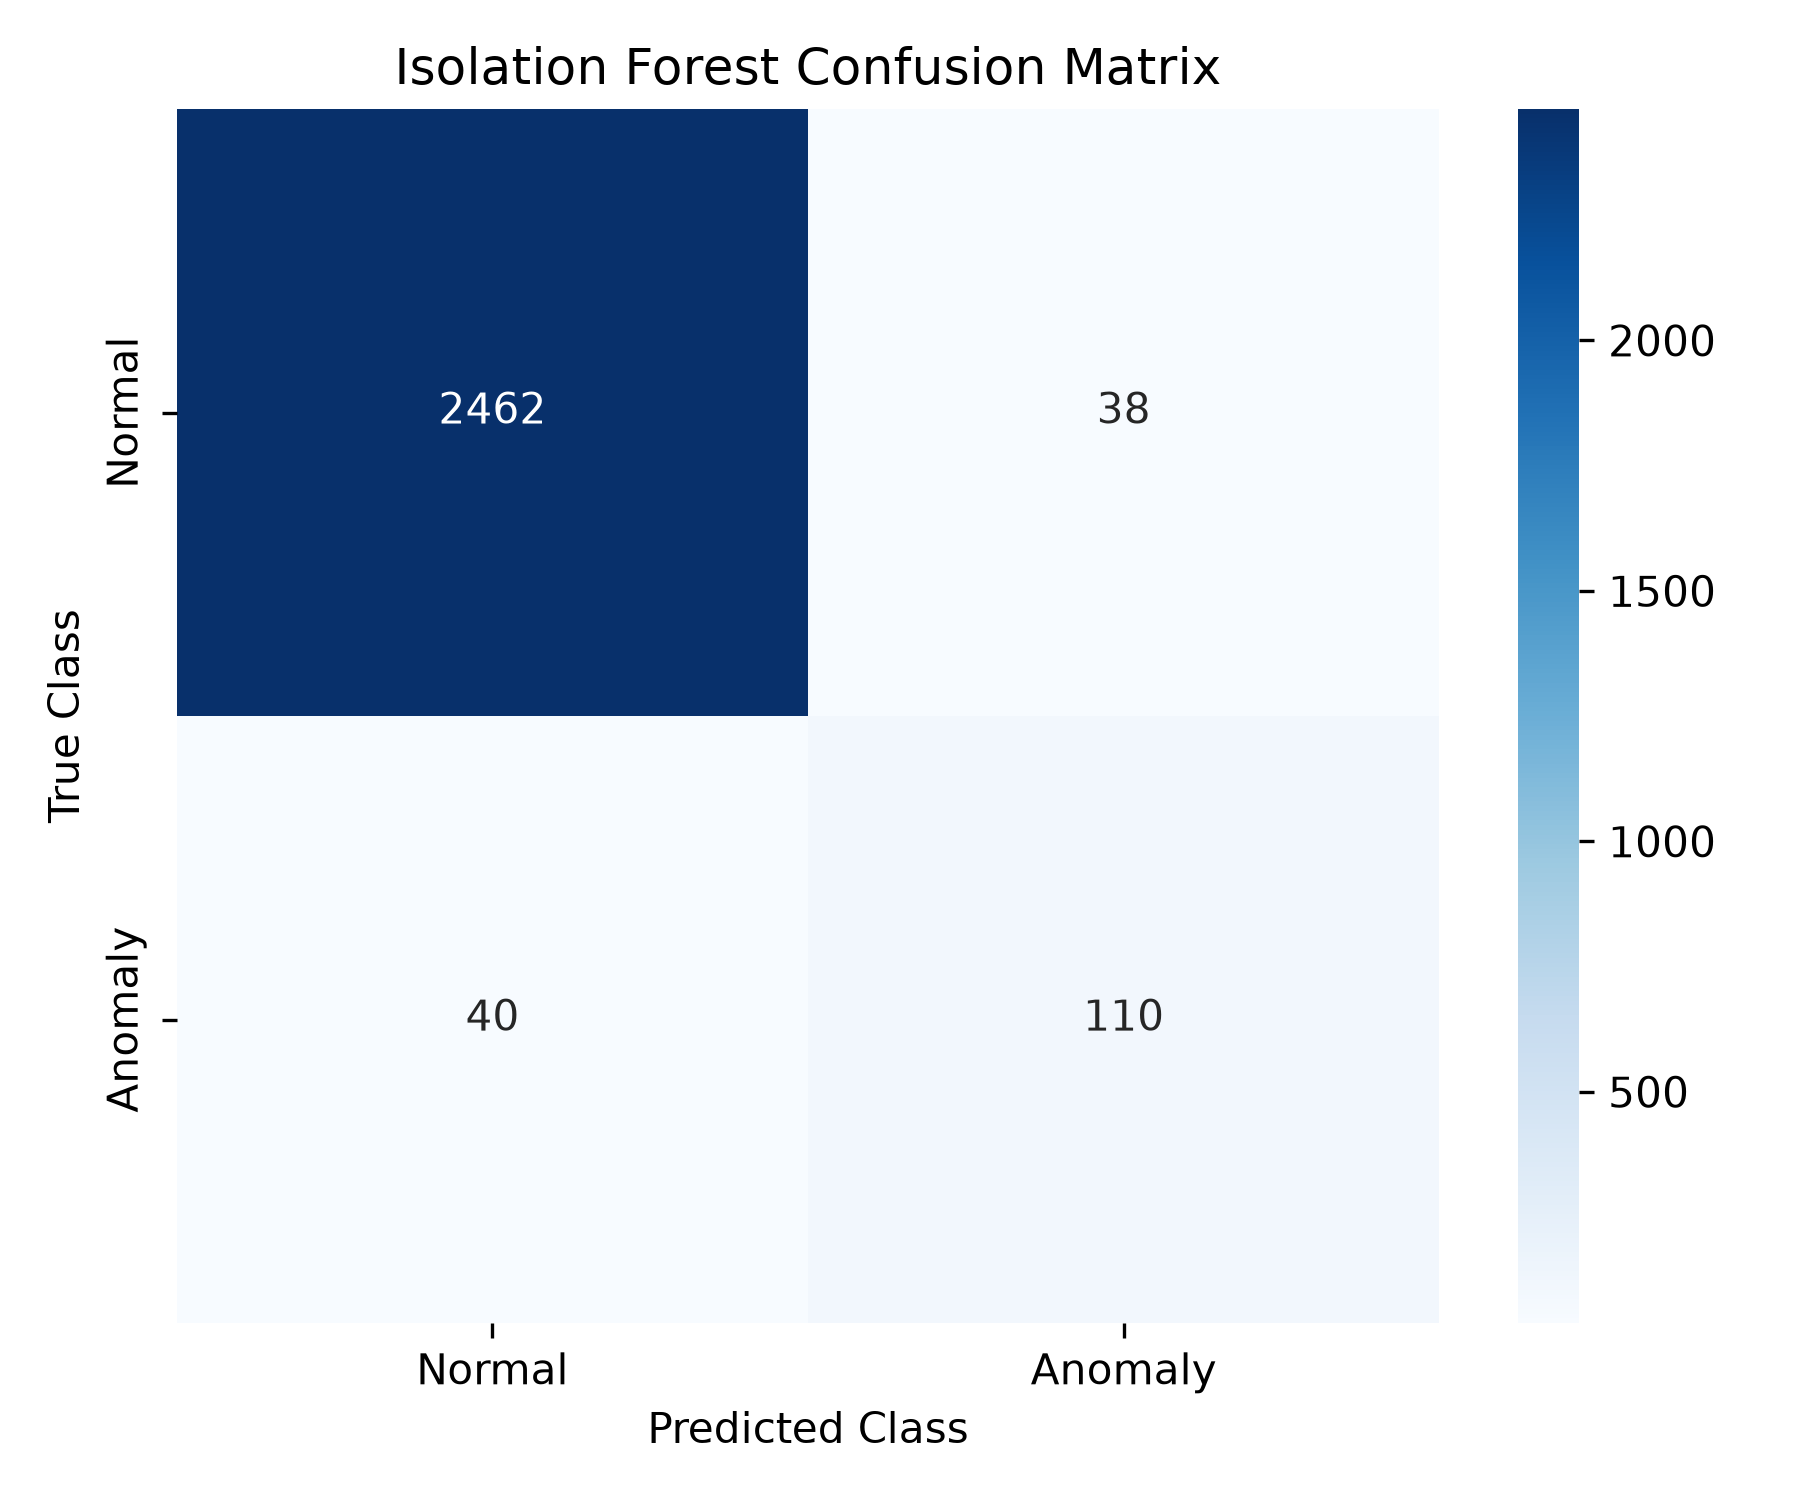
\includegraphics[width=\textwidth]{confusion_matrix.png}
    \caption{Empirical Confusion Matrix of Anomaly Classifier.}
    \label{fig:confusion}
\end{minipage}
\hfill
\begin{minipage}{0.48\columnwidth}
    \centering
    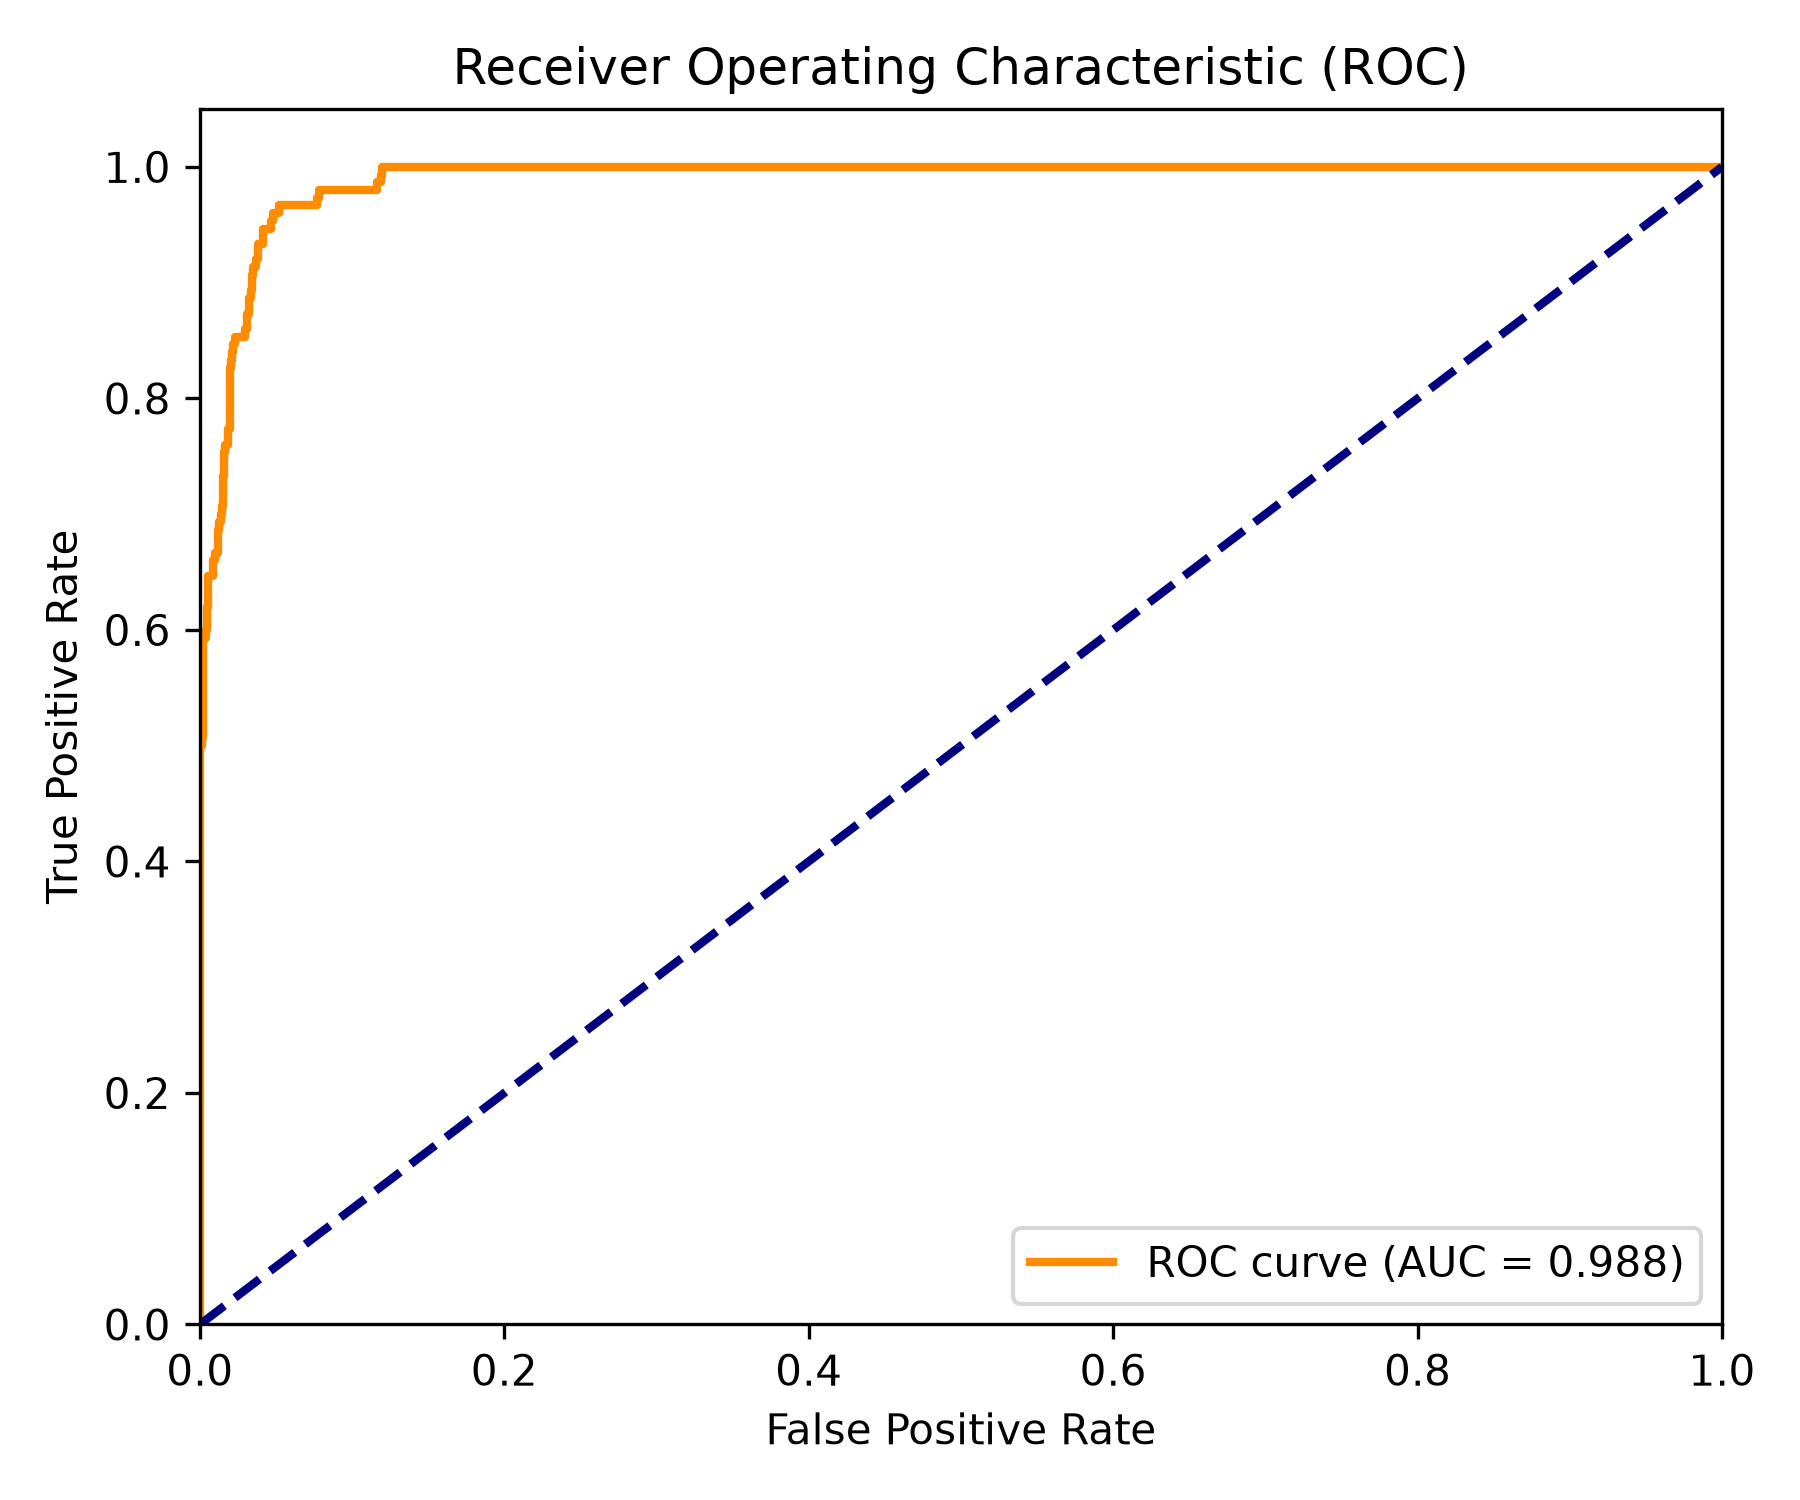
\includegraphics[width=\textwidth]{roc_curve.png}
    \caption{ROC Curve of Isolation Forest (AUC = 0.9885).}
    \label{fig:roc}
\end{minipage}
\end{figure}

Fig. \ref{fig:confusion} and Fig. \ref{fig:roc} illustrate the dominant diagonal classification and near-optimal ROC discriminative curve generated during training evaluation.

\subsection{Biometric Verification Sensitivity}
Table \ref{tab:biometric} summarizes pairwise Euclidean distances across live sessions. Setting $\tau_{\text{match}} = 0.76$ provides clean separation between genuine voters ($d \le 0.725$) and unauthorized imposters ($d \ge 0.819$).

\begin{table}[htbp]
\caption{Pairwise Biometric Distance Calibration Across Camera Sessions}
\label{tab:biometric}
\centering
\renewcommand{\arraystretch}{1.25}
\resizebox{\columnwidth}{!}{%
\begin{tabular}{|l|c|c|c|}
\hline
\textbf{Comparison Pairing Type} & \textbf{Distance Range ($d$)} & \textbf{Classification} & \textbf{Empirical Decision} \\
\hline
Intra-Person (Identical session) & $[0.000, 0.240]$ & Genuine & Verified ($\tau \le 0.76$) \\
\hline
Intra-Person (Lighting / Glasses) & $[0.462, 0.725]$ & Genuine & Verified ($\tau \le 0.76$) \\
\hline
Inter-Person (Similar room / scene) & $[0.819, 1.010]$ & Imposter & Rejected / Flagged ($d > 0.76$) \\
\hline
Inter-Person (Distinct subjects) & $[1.292, 1.447]$ & Imposter & Rejected / Blocked ($d > 0.76$) \\
\hline
\end{tabular}%
}
\end{table}

\subsection{Ledger Verification Latency}
Integrity verification using \texttt{scripts/verify\_ledger\_cli.js} verified 1,000 sequential ballots in $42.5\text{ ms}$. Tamper injection tests confirmed that altering a single recorded vote broke chaining within $1.1\text{ ms}$, reliably identifying the corrupted block index.

\section{Security Analysis \& Threat Model}
Table \ref{tab:stride} summarizes the platform's defense coverage evaluated against Microsoft's STRIDE framework \cite{hernan2006threat}.

\begin{table}[htbp]
\caption{STRIDE Threat Model Evaluation and Security Countermeasures}
\label{tab:stride}
\centering
\renewcommand{\arraystretch}{1.3}
\resizebox{\columnwidth}{!}{%
\begin{tabular}{|c|l|p{5.5cm}|}
\hline
\textbf{Category} & \textbf{STRIDE Threat} & \textbf{System Architectural Defense \& Mitigation} \\
\hline
\textbf{S} & Spoofing & 128-d DCT/Sobel face verification ($d \le 0.76$) paired with temporal multi-frame liveness and HMAC-salted email OTP. \\
\hline
\textbf{T} & Tampering & Backward-linked SHA-256 cryptographic hash chaining; standalone CLI auditor verifies block integrity in $<45\text{ ms}$. \\
\hline
\textbf{R} & Repudiation & Deterministic cryptographic receipt tokens (\texttt{REC-}$\dots$) and immutable append-only audit trail logs. \\
\hline
\textbf{I} & Information Disclosure & Strict schema decoupling: \texttt{VoteRecord} (eligibility) is mathematically isolated from anonymized \texttt{Ballot}. \\
\hline
\textbf{D} & Denial of Service & Layered token-bucket rate limiting ($200\text{ req}/15\text{ min}$) and real-time Isolation Forest bot-burst mitigation. \\
\hline
\textbf{E} & Elevation of Privilege & Role-Based Access Control (RBAC) enforced via cryptographically signed stateless JWT claims at API gateway. \\
\hline
\end{tabular}%
}
\end{table}

\section{Discussion, Limitations, and Ethics}

\subsection{Biometric Privacy and Right to Erasure}
Storing raw facial photographs on centralized servers creates an attractive target for adversaries \cite{ratha2001enhancing}. Our architecture mitigates this by converting images to 128-dimensional frequency representations with the DC coefficient removed ($D(0, 0) = 0.0$), rendering inverse facial reconstruction ill-posed. Furthermore, compliance with GDPR Article 17 \cite{gdpr2016regulation} is implemented through the self-service endpoint \texttt{DELETE /api/v1/auth/me}, permanently erasing biometric embeddings while preserving anonymized hash-chain ballots.

\subsection{Non-Blocking Triage vs. Disenfranchisement}
Rejecting votes automatically on algorithmic anomaly signals introduces the risk of algorithmic disenfranchisement \cite{eubanks2018automating}. Our asymmetric non-blocking triage ensures that flagged ballots are sealed to the ledger and included in provisional counts, while \texttt{FraudAlert} records are archived for post-election administrative review.

\subsection{System Limitations}
The platform assumes client browser sandbox integrity and cannot detect kernel-level virtual camera drivers injecting synthetic video streams \cite{mirsky2021creation}. Remote voting also remains susceptible to physical terminal coercion \cite{chaum2004secret}, which polling stations prevent.

\section{Conclusion and Future Work}
In this paper, we presented an AI-augmented secure online voting architecture combining the MERN web stack with an applied machine learning microservice and a cryptographic hash-chained ballot ledger. By unifying 128-dimensional facial biometrics, eyeglass-resilient liveness detection, and an unsupervised Isolation Forest anomaly detector, the platform mitigates automated bot attacks, presentation attacks, and database tampering while preserving secret ballot anonymity. Experimental evaluation confirmed 97.06\% classification accuracy and an ROC-AUC of 0.9885 with a 1.52\% false positive rate.

Future extensions will incorporate Zero-Knowledge Succinct Non-Interactive Arguments of Knowledge (zk-SNARKs) \cite{bensasson2014succinct} for client-side biometric matching, secure Multi-Party Computation (MPC) \cite{cramer2015secure} for distributed ballot tallying, and hardware-bound FIDO2/WebAuthn credentials.

\bibliographystyle{IEEEtran}
\bibliography{references}

\end{document}
